\section{Model}
\label{sec:model}

\setlength{\tabcolsep}{2pt}
\begin{figure*}
\begin{center}
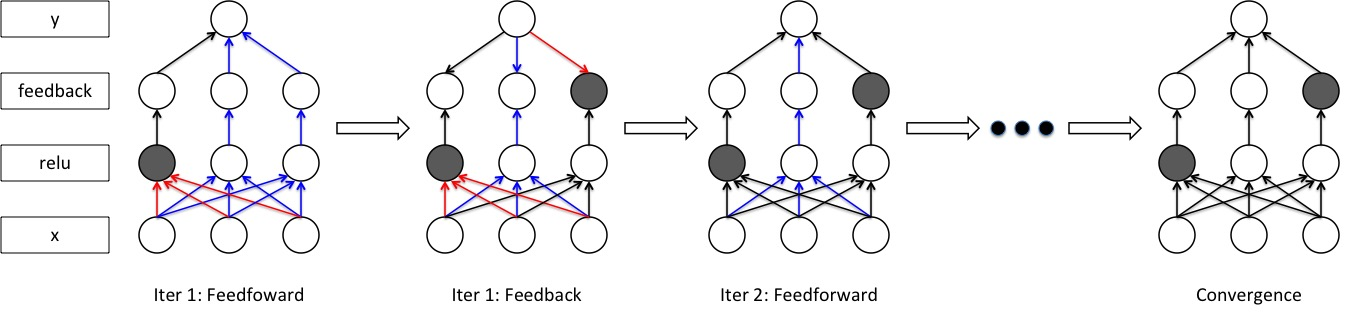
\includegraphics[width=0.95\linewidth]{figs/model/model}
% \vspace{-10pt}
\caption{Illustration of our feedback model and its inference process. At the first iteration, the model performs as a feedforward neural net. After then, the neurons in the feedback hidden layers update their activation status to maximize the confidence output of the target top neuron. This process continues until convergence. (We show only one layer here, but the feedback layers can be tacked in the deep ConvNet.) Better viewed in color.}
\label{fig:model}
% \vspace{-30pt}
\end{center}
\end{figure*}

We first review the current state-of-the-art feedforward Deep Convolutional Neural Networks (CNNs) architecture and then propose our feedback model on top of that. 

\subsection{Review of Convolutional Neural Networks}
The most recent state-of-the-art deep CNNs~\cite{Simonyan2014Very} consist of many stacked feedforward layers, including convolutional, rectified linear units (ReLU) and max-pooling layers. For each layer, the input $\mathbf{x}$ can be an image or the output of a previous layer, consisting of $C$ input channels of width $M$ and height $N$: $\mathbf{x} \in \mathcal{R}^{M \times N \times C}$. The output $\mathbf{y}$ consists of a set of $C'$ output channels of width $M'$ and height $N'$: $\mathbf{y} \in \mathcal{R}^{M' \times N' \times C'}$. 

\textbf{Convolutional Layer:} 
The convolution layer is used to extract different features of the input. The convolutional layer is parameterized by $C'$ filters with every filter $\mathbf{k} \in \mathcal{R}^{K \times K \times C}$.
\begin{equation}
\mathbf{y}_{c'} = \sum_{c=1}^C \mathbf{k}_{c'c} * \mathbf{x}_c,\ \forall c'
\end{equation}

\textbf{ReLU Layer:}
The ReLU layer is used to increase the nonlinear properties of the decision function and of the overall network without affecting the receptive fields of the convoluional layer.
\begin{equation}
\mathbf{y} = \max (\mathbf{0}, \mathbf{x})
\label{eq:relu}
\end{equation} 

\textbf{Max-Pooling Layer:}
The max-pooling layer is used to reduce the dimensionality of the output and variance in deformable objects to ensure that the same result will be obtained even when image features have small translations. The max-pooling operation is applied for every pixel $(i,j)$ around its small neighborhood $\mathcal{N}$.
\begin{equation}
y_{i,j,c} = \max_{u,v \in \mathcal{N}} x_{i+u, j+v, c},\ \forall i, j, c
\label{eq:max-pool}
\end{equation}

\begin{comment}
\textbf{Fully Connnected Layer:} The fully connected layer is parameterized by the production matrix with $W \in \mathcal{R}^{M'N'C' \times MNC}$. 
Finally, a few fully connected layers (normally with drop-out) is stacked on top of the convolutional outputs to compute the scores of every class. 
\begin{equation}
\vec{y}_l = W_l^T  \vec{y}_{l-1}
\end{equation}
\end{comment}

\subsection{Re-interpretion of ReLU and Max-Pooling}
We can re-interpret ReLU and max-pooling layers as components for feature selection when introducing the binary activation variables $\mathbf{z}: \mathbf{z} \in \{0, 1\}$. 

For the ReLU layer, $\mathbf{z}$ is the same size as the input $\mathbf{x}$. 

while for the max-pooling, $\mathbf{z}$ is similar as a set of location variant filters. 

Given that Equations~\ref{eq:relu} and~\ref{eq:max-pool} can be re-interpreted.

For the ReLU layer, $\mathbf{y} = \mathbf{z} \circ \mathbf{x}$, where $\circ$ is the element wise product (Hadamard product). The element value in $\mathbf{z}$ is determine by $\mathbf{x}$ as the property of ReLU.

For the max-pooling layer, $\mathbf{y} = \mathbf{z} * \mathbf{x}$, where $*$ is the convolution operation. The element value in $\mathbf{z}$ is determined by $\mathbf{x}$ as the property of max-pooling.

For both layers, the $\max()$ functions are replaced with linear operations between the inputs and binary hidden variables. The binary latent variables performs as feature selection. However, the values of the latent variables $\mathbf{z}$ are completely determined by the bottom-up input $\mathbf{x}$, meaning that the feature selection based on bottom-up. 

During the feedforward process, since the middle layers have no idea about what is going on on the top layers, they have to keep the information passed from bottom layers as much as possible. Hence the final layer features computed for classifcation are sharable among all classes. It can be imagined that when ConvNets compute the middle layer features, it tries to make the largest possible information pass through the network. However, These features are stationary and even when there provide with prior information about top level neurons, the features won't change themselves.

However, in order to recognize the image, the middle level layers are designed to provide all possible information for the final layer to classify. This works well when there is only one salient object in the image. However when people care about different aspects in the images, the same feature may not be appropriate all the time. 

Since the model open all the gates for the gates for all information to pass, when we are targeted on a paticular semantic labels, we want to turn off those gates that provide irrelavant information for seeing that object. This top-down message will be utilized to turn off those relu.

We model the top down as another type of activation variable, similar as ReLu. However, this unit activates based on the the overall information of bottom-up responses and top-down messages. 

To understand the model, we allow each ReLU neuron to either turn on, turn off, or pass a proportion of the information computed from the convolutional layer, in order to maximially interpret the image as the target class.

\subsection{Adding the Feedback Layer}
We model a feedback layer on top of the relu layers to improve the activation felxibility, that the feedback neuron activation variables depend on the weights from high level targets. When combined with ReLU layer, the two layers not only capture on the bottom-up features but also top-down weights passed from the target neuron. Figure.~\ref{fig:model} illustrates the architecture of our model and the inference process. 

\subsection{Updating Hidden Neurons in Feedback Layers}
Given an image $I$ and a neural network with learned parameters $w$, we optimize the target neuron output by jointly reasoning neuron activiations $\mathbf{z}$ over all the hidden layers. In particular, if the target neuron is the class node in the top layer, we optimize the class score $s_k$ by looking for the reorganization of hidden neuron activations on the ReLU layer:
\begin{equation}
\begin{aligned}
  \max_z s_k(I, z) \\
  s.t.\ z \in \{0, 1\}
\end{aligned}
\end{equation}

This leads to an integer programming problem, which is a NP-hard problem given the current deep convolutional neural net structure. To obtain a good solution, we apply a linear relaxation.

In the linear relaxation, we rephrase the problem as:
\begin{equation}
\begin{aligned}
  \max_h S_c(I_0, h) \\
  s.t.\ 0 \leq h_i \leq 1
\end{aligned}
\end{equation}

\subsection{Implementation Details}
In real implementation, we set the feedback layer on top of every ReLU layer except those taking the fully connected layers as inputs. We suspect the fully connected layers learn more embedding spaces rather than paticular parts compared to convolutional layers. We set learning rate of hidden activations to 0.1 and update the neurons of all the feedback layers simultaneously. Each iteration performs a feedforward step of the neural net and a backpropagation step to send back gradients. This process usually converges in 10 to 50 iterations. After that, we set a hidden neuron activation to 1 if its value is greater than 0.5 and 0 if smaller. 
